%%%%%%%%%%%%%%%%%%%%%%%%%%%%%%%%%%%%
% Header                           %
%%%%%%%%%%%%%%%%%%%%%%%%%%%%%%%%%%%%
% 
% Revisions: 2017-04-10 Martin Rädel <martin.raedel@dlr.de>
%                       Initial draft
%               
% Contact:   Martin Rädel,  martin.raedel@dlr.de
%            DLR Composite Structures and Adaptive Systems
%          
%                                 __/|__
%                                /_/_/_/  
%            www.dlr.de/fa/en      |/ DLR
% 
%%%%%%%%%%%%%%%%%%%%%%%%%%%%%%%%%%%%
% Content                          %
%%%%%%%%%%%%%%%%%%%%%%%%%%%%%%%%%%%%

If no native Linux-based operating system is available on a device it is possible to install a Linux distribution inside a virtual machine. The device used to install the virtual machine in is called the host in the description.

In case you have a native Linux operating system on your device you can skip the following steps and go to chapter \ref{sec:Peridigm_Linux_Installation}.

\leveldown{Download Linux Distribution} \label{sec:VirtualBox_Download_Linux_Distribution}

For \marktool{\toolname} we need a Linux distribution for the installation inside the virtual machine. Here, \marktool{\opensusename} is used. To download the latest version of \marktool{\opensusename} go to:

\href{\opensuseaddress}{\opensuseaddress}

In the top bar of the homepage go to the download section and choose \textit{Latest stable release}. On the newly loaded page choose to download the DVD image as installation medium and perform the download onto your device. Beware, the image is quite big.

\levelstay{Install the virtual machine}

\leveldown{Download and install virtualization software}

For the current case \marktool{\virtualboxname} is chosen as the virtualization environment. \marktool{\virtualboxname} is available for enterprise and home use and is freely available for both use-cases as Open Source Software under the terms of the GNU General Public License (GPL) version 2. The following chapter describes the setup of the then current version of \marktool{\opensusename} in a \marktool{\virtualboxname} on your host operation system. \marktool{\virtualboxname} is currently available for

\begin{itemize}[noitemsep, nolistsep, columns=4]
 \item Windows
 \item OSX
 \item Linux
 \item Solaris
\end{itemize}

host operating systems. The current release of \marktool{\virtualboxname} is available from:

\href{\virtualboxaddress}{\virtualboxaddress}

Go to the download section and choose the installer for your host operating system. The following description is valid for a Windows host and is tested for the 64bit variant of Windows 7. After the download execute the binary installer and follow the instructions of the setup wizard. In the custom setup step simply let all selected items enabled. Afterwards simply complete the wizard.

\begin{figure}[htbp]
\centering
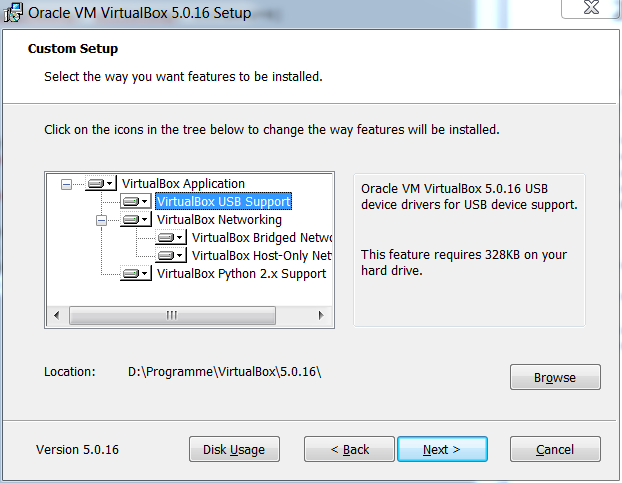
\includegraphics[scale=\screenshotscalefac]{Figures/VirtualBox_Install_Custom_Setup}
\end{figure}

During the installation simply answer the following questions with \textit{install} to allow access on the devices for the virtual machine.

\begin{figure}[htbp]
  \begin{subfigure}{\linewidth}
    \centering
    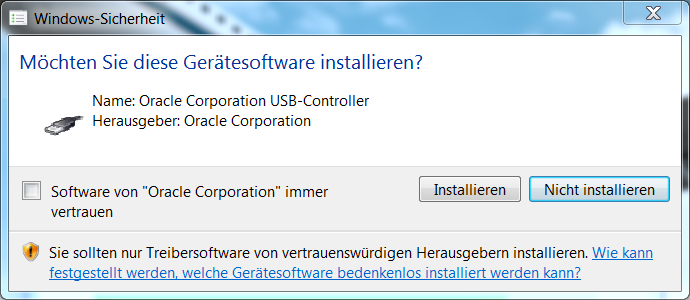
\includegraphics[scale=\screenshotscalefac]{Figures/VirtualBox_Install_Allow_USB}
    \caption{Install USB-Controller}
    \label{fig:VirtualBox_Install_Allow_USB}
  \end{subfigure}%
\vspace{1ex}\\
% \end{figure}
% 
% \begin{figure}[htbp]
%   \ContinuedFloat
  \begin{subfigure}{\linewidth}
    \centering
    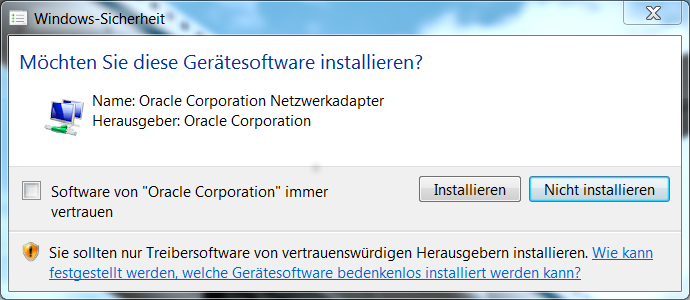
\includegraphics[scale=\screenshotscalefac]{Figures/VirtualBox_Install_Allow_Network_Adapter}
    \caption{Install network adapter}
    \label{fig:VirtualBox_Install_Allow_Network}
  \end{subfigure}%
  \vspace{1ex}\\
  \begin{subfigure}{\linewidth}
    \centering
    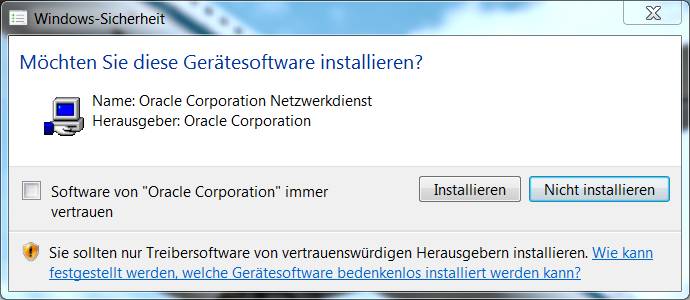
\includegraphics[scale=\screenshotscalefac]{Figures/VirtualBox_Install_Allow_Network_Service}
    \caption{Install network service}
   \label{fig:VirtualBox_Install_Allow_Network_Service}
  \end{subfigure}%
  \caption{Allow \marktool{\virtualboxname} access to devices}
  \label{fig:VirtualBox_Install_Allow}
\end{figure}

\clearpage

\levelstay{Create the virtual machine}

After the installation is complete start the \marktool{\virtualboxname} Manager.

\begin{figure}[htbp]
\centering
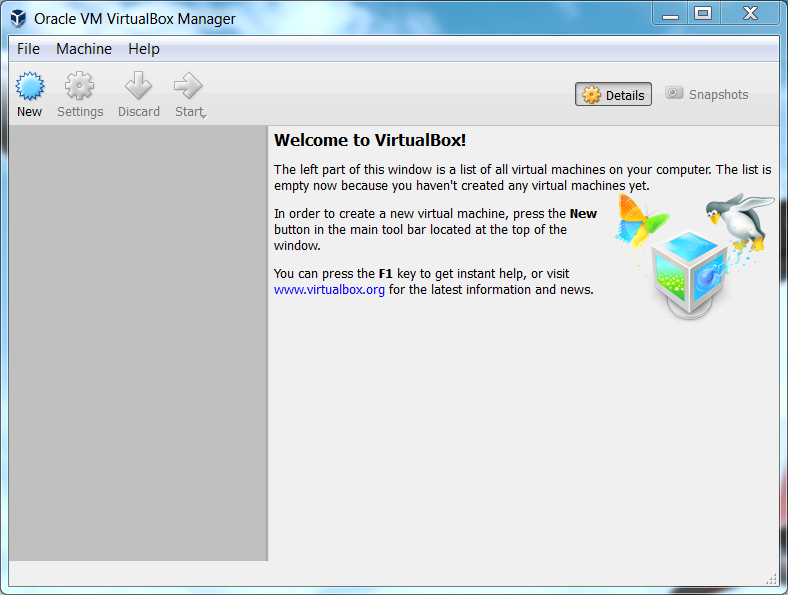
\includegraphics[scale=\screenshotscalefac]{Figures/VirtualBox_Start_Menu}
\end{figure}

Before we create a new virtual machine

\begin{itemize}[noitemsep]
 \item From the menu bar: Click \textit{File}
 \item Click \textit{Preferences}
 \item In the \textit{General} tab select the \textit{Default Machine Folder} to be a folder on a harddrive with sufficient amount of free memory to handle your virtual machine size, here 200GB\\
 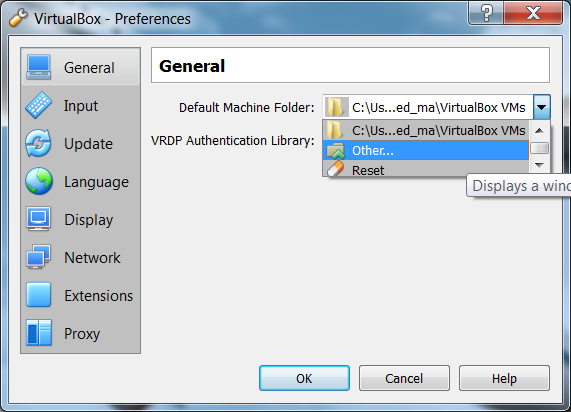
\includegraphics[scale=\screenshotscalefac]{Figures/VirtualBox_Preferences_General}
 \item Close the Preferences windows with a click in \textit{Ok}
\end{itemize}

Now we can create a new virtual machine. Click \textit{New} in the \marktool{\virtualboxname} Manager main window. A dialog appears that guides you through the setup of the virtual machine.

\begin{enumerate}[noitemsep]
  \item Select the virtual machine name, type and version
    \begin{itemize}
      \item Choose a name that includes the version \& the selection automatically jumps to your choice
      \item Choose the 64bit variant\\
      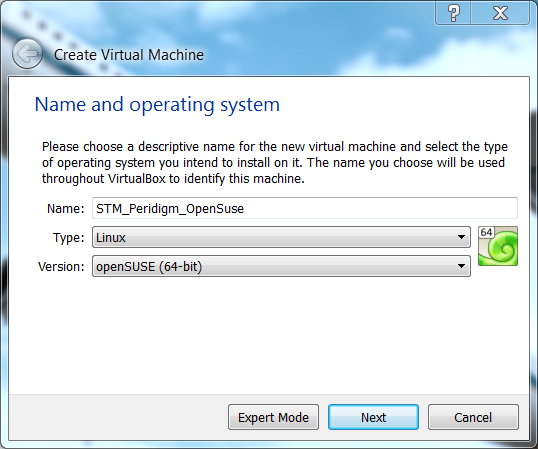
\includegraphics[scale=\screenshotscalefac]{Figures/VirtualBox_Create_VirtualMachine_Name_OS}
      \item A new folder with your chosen name is created in the directory you specified in the \textit{General} tab of the \textit{Preferences} toolbar menu
      \item Click \textit{Next}
    \end{itemize}
 \item Set the amount of RAM you grant your virtual machine
    \begin{itemize}
      \item The more RAM \marktool{\toolname} has available the better
      \item But your host operating system also still needs some RAM left to work with
      \item Choose an integer multiple of 1024 as amount of RAM
      \item Leave the host operating system at least 2GB of RAM
      \item You can select values in the red marked area\\
      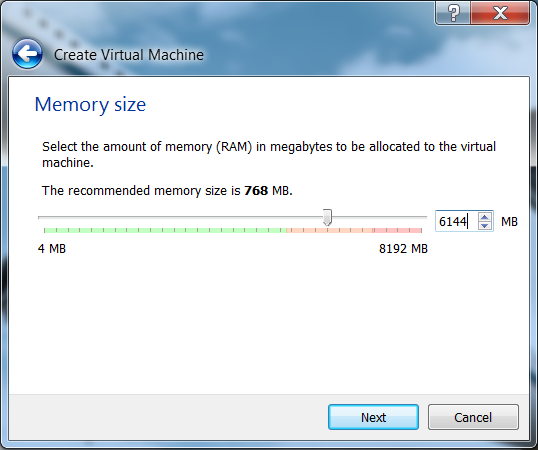
\includegraphics[scale=\screenshotscalefac]{Figures/VirtualBox_Create_VirtualMachine_RAM}
      \item Click \textit{Next}
    \end{itemize}
 \item Create a virtual hard disk to install your distribution on
    \begin{itemize}
      \item Here we select the \textit{Create a virtual hard disk now} option\\
      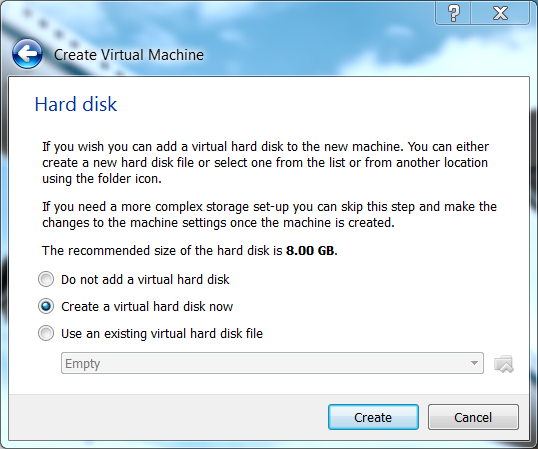
\includegraphics[scale=\screenshotscalefac]{Figures/VirtualBox_Create_VirtualMachine_Harddisk}
      \item Click \textit{Create}
      \item Select \textit{VMDK (Virtual Machine Disk)} to allow use of this virtual hard disk in other virtualization tools like VMWare.\\
      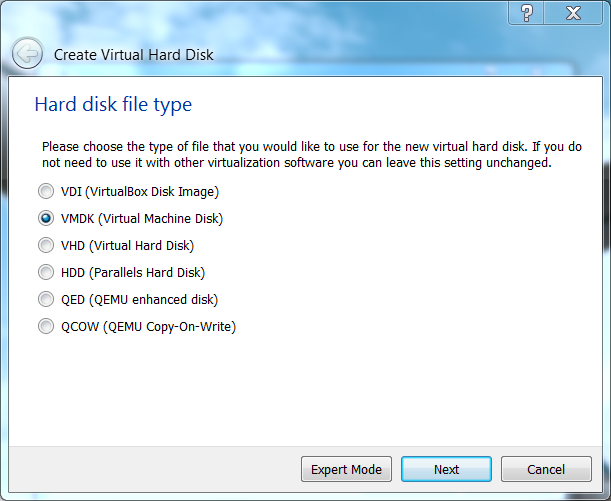
\includegraphics[scale=\screenshotscalefac]{Figures/VirtualBox_Create_VirtualMachine_Harddisk_File_Type}
      \item Click \textit{Next}
      \item Select \textit{Fixed size}
      \item Do not select \textit{Split into files less than 2GB}\\
      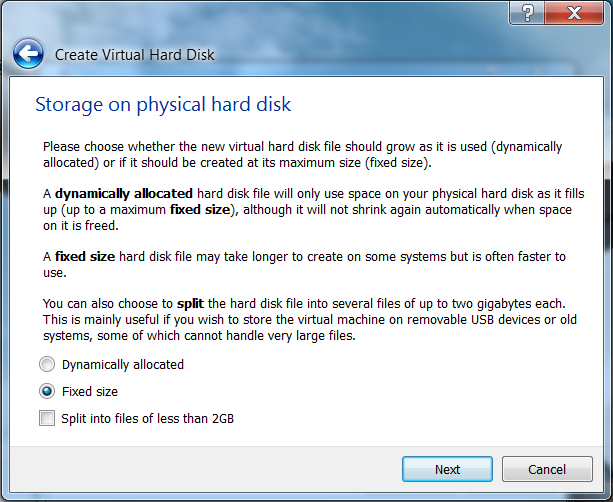
\includegraphics[scale=\screenshotscalefac]{Figures/VirtualBox_Create_VirtualMachine_Harddisk_Storage_Type}
      \item Click \textit{Next}
      \item Setup virtual hard disk name and size
      \item By default the name is identical to the virtual machine name
      \item If you click the folder button you can change the location of the virtual hard disk file. By default it is saved in your virtual machine folder in the directory specified in the \textit{General} tab of the \textit{Preferences} toolbar menu
      \item Set the size of the virtual hard disk to the amount you want and have free, here 200GB. Despite being saved in binary format, \marktool{\toolname} result files can be quite big and for explicit time integration a lot of them are created. Despite a Linux distribution does not need nearly as much hard disk space as a Windows installation, at least 120GB are proposed as virtual hard disk size.\\
      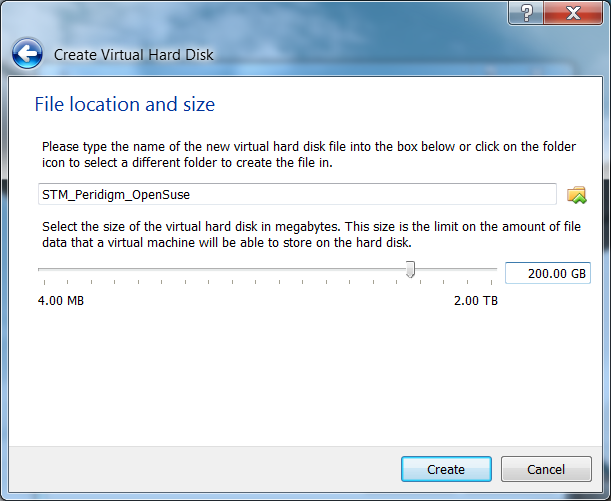
\includegraphics[scale=\screenshotscalefac]{Figures/VirtualBox_Create_VirtualMachine_Harddisk_Location}
      \item Click \textit{Create}
      \item Wait for the creation to finish
      \item Afterwards you have a new virtual machine\\
      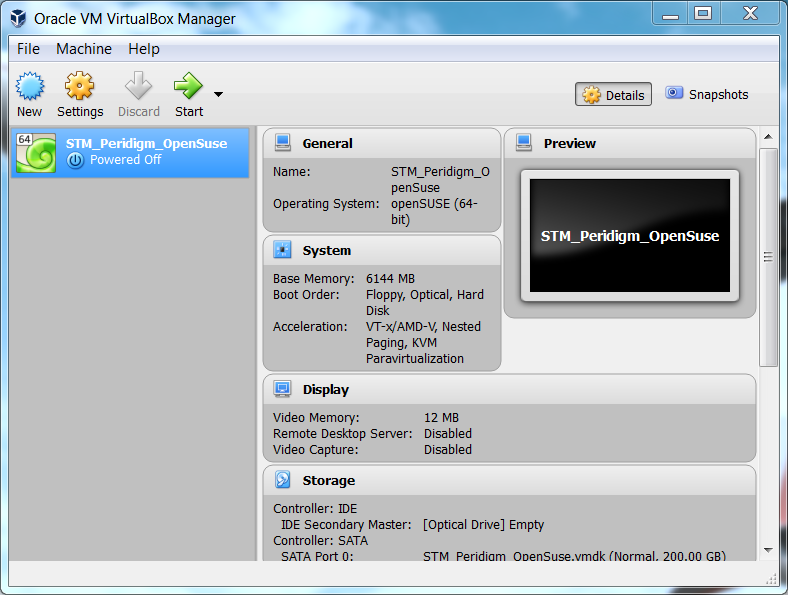
\includegraphics[scale=\screenshotscalefac]{Figures/VirtualBox_Create_VirtualMachine_Finished}
    \end{itemize}
  \item \label{enum:Virtual_Machine_Settings}Before we install the Linux distribution inside the virtual machine, we have to configure some settings
  \begin{itemize}
    \item Select the newly created virtual machine and click \textit{Settings}
    \item In the \textit{General} tab
    \begin{itemize}
      \item Select \textit{Advanced}
      \item Select:%\\
      \begin{tabular}[t]{ll}
      \textit{Shared Clipboard}	& Bidirectional	\\
      \textit{Drag'n'Drop}	& Bidirectional	\\
      \end{tabular}\\
      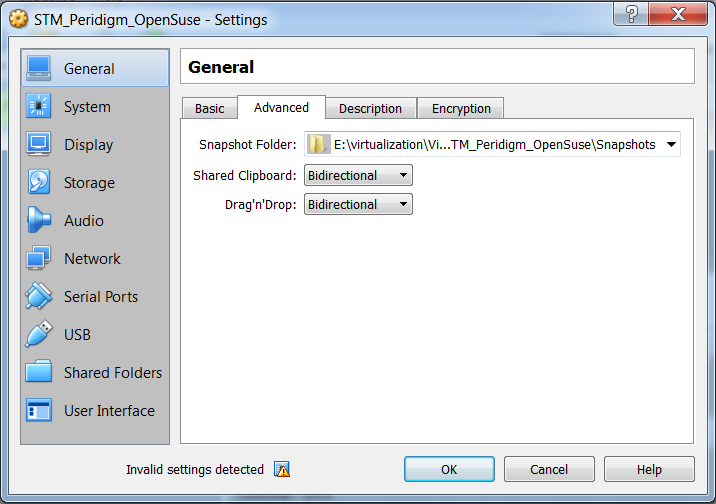
\includegraphics[scale=\screenshotscalefac]{Figures/VirtualBox_VirtualMachine_Settings_General_Advanced}
    \end{itemize}
    \item Ignore the warning about \textit{Invalid settings detected} if this is only a RAM issue
    \item In the \textit{System} tab
    \begin{itemize}
      \item Select \textit{Processor}
      \item Set \textit{Processor(s)} to your preferred value
      \item At least one CPU should be left for the host machine\\
      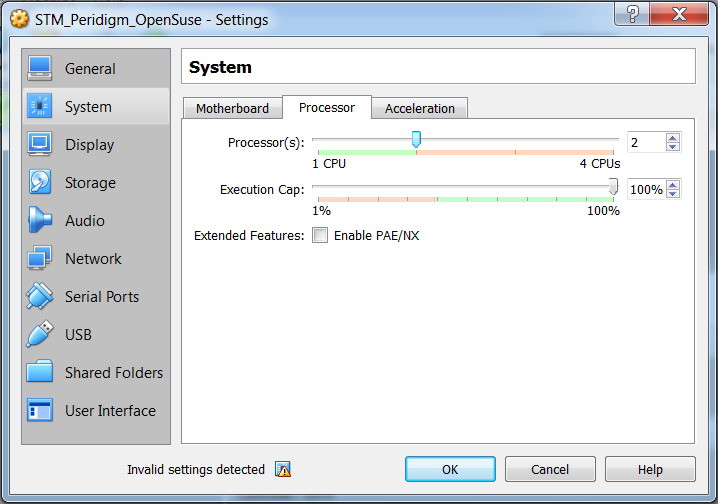
\includegraphics[scale=\screenshotscalefac]{Figures/VirtualBox_VirtualMachine_Settings_System_Processor}
    \end{itemize}
    \item In the \textit{Display} tab
    \begin{itemize}
      \item Select \textit{Screen}
      \item Set \textit{Video Memory} to maximum\\
      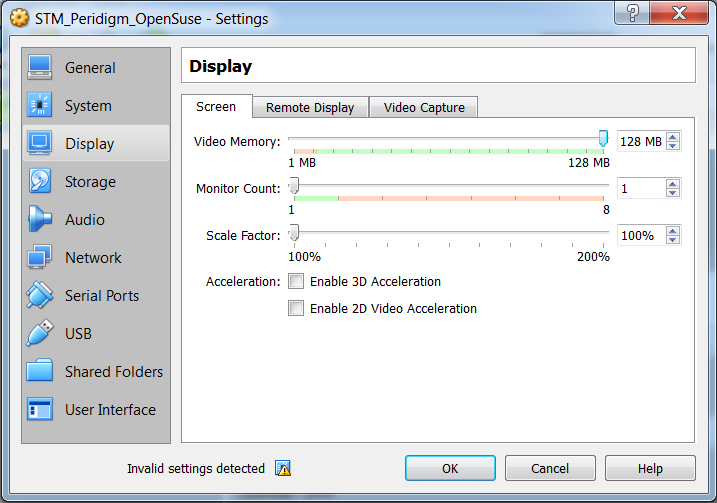
\includegraphics[scale=\screenshotscalefac]{Figures/VirtualBox_VirtualMachine_Settings_Display_Screen}
    \end{itemize}
%     \item In the \textit{Shared Folders} tab
%     \begin{itemize}
%       \item Click the + folder button on the right
%       \item In \textit{Folder Path:} create or add a transfer folder between your host system and your virtual machine\\
%       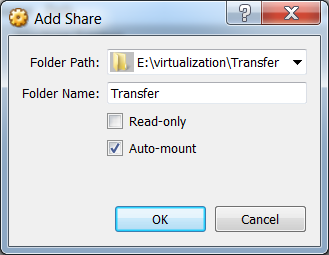
\includegraphics[scale=\screenshotscalefac]{Figures/VirtualBox_VirtualMachine_Settings_SharedFolders_Add}
%       \item Select \textit{Auto-mount}\\
%       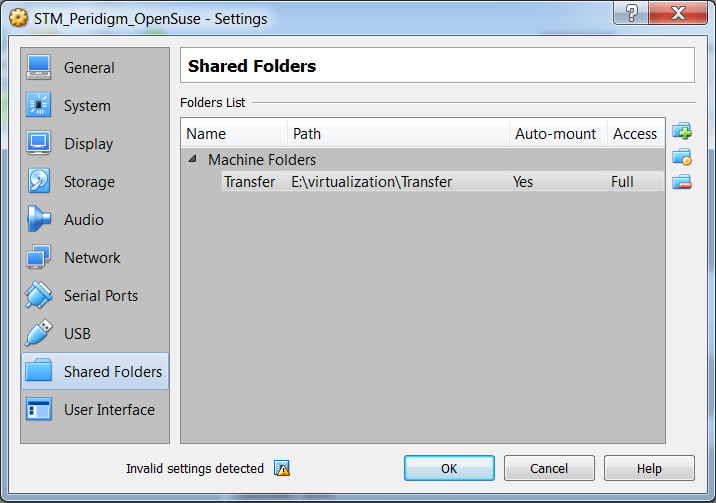
\includegraphics[scale=\screenshotscalefac]{Figures/VirtualBox_VirtualMachine_Settings_SharedFolders}
%     \end{itemize}
  \item Click \textit{OK}
  \end{itemize}
\end{enumerate}

All modifications to the virtual machine preferences in step \ref{enum:Virtual_Machine_Settings} can be modified after the installation of the virtual machine distribution in case the virtual machine is shut down.

\levelstay{Create a shared folder between host and virtual machine}



\begin{enumerate}[noitemsep]
  \item In the host operating system:
    \begin{itemize}
     \item Open a Windows Explorer
     \item Create a shared folder for the file exchange between the host and the virtual machine operating system anywhere it suits you or use an existing one, here the shared folder is \verb+E:\virtualization\Transfer+
     \item Right-Click the newly created folder and click \textit{Properties}
     \item In the \textit{Shared Folders/Freigabe} tab
      \begin{itemize}
	\item Click on \textit{Freigabe}
	\item In the dialog appearing click on the combobox arrow and select \textit{Anyone/Jeder}
	\item Click \textit{Freigabe}
	\item Click \textit{Close}
      \end{itemize}
      \item Be aware that the folder is visible in your whole network
    \end{itemize}
  \item Inside the virtual box manager:
    \begin{itemize}
      \item Select the newly created virtual machine and click \textit{Settings}
      \item In the \textit{Shared Folders} tab
      \begin{itemize}
	\item Click the + folder button on the right
	\item In \textit{Folder Path:} create or add a transfer folder between your host system and your virtual machine\\
	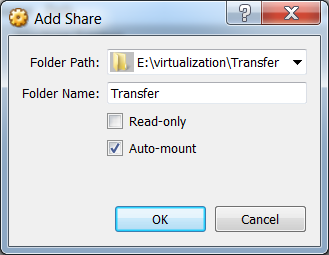
\includegraphics[scale=\screenshotscalefac]{Figures/VirtualBox_VirtualMachine_Settings_SharedFolders_Add}
	\item Select \textit{Auto-mount}\\
	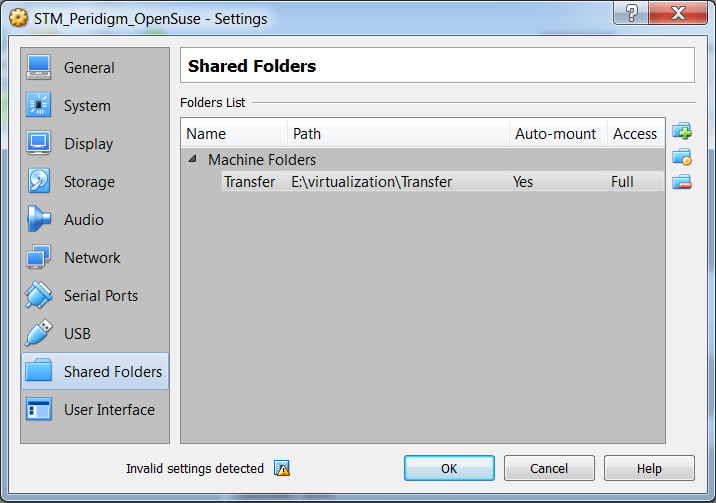
\includegraphics[scale=\screenshotscalefac]{Figures/VirtualBox_VirtualMachine_Settings_SharedFolders}
      \end{itemize}
    \item Click \textit{OK}
    \end{itemize}
\end{enumerate}

\levelstay{Install the operating system in the virtual machine}

Now, we can install the virtual machine operating system:

\begin{enumerate}[noitemsep]
 \item Start the installation
 \begin{itemize}
   \item Select the virtual machine in the \marktool{\virtualboxname} Manager and click \textit{Start}\\
   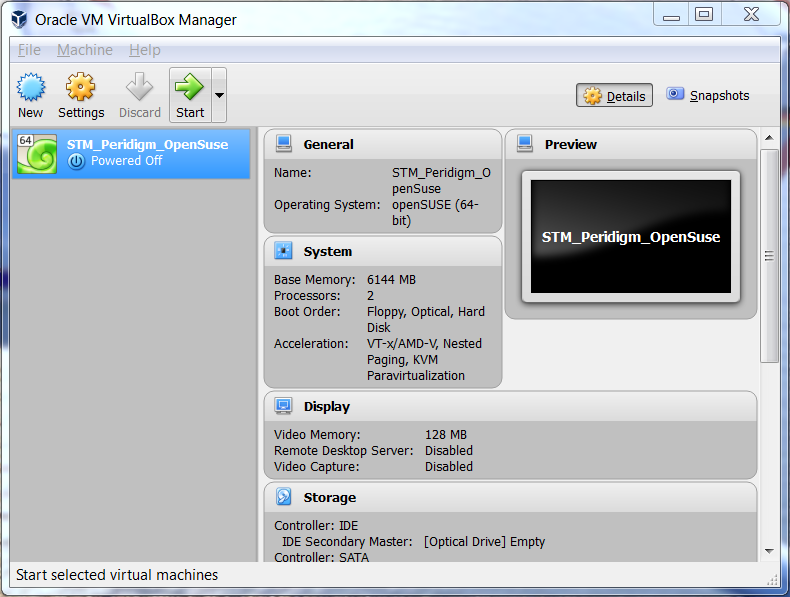
\includegraphics[scale=\screenshotscalefac]{Figures/VirtualBox_VirtualMachine_OperatingSystem_Start}
   \item Select the \marktool{\opensusename} image from section \ref{sec:VirtualBox_Download_Linux_Distribution}\\
   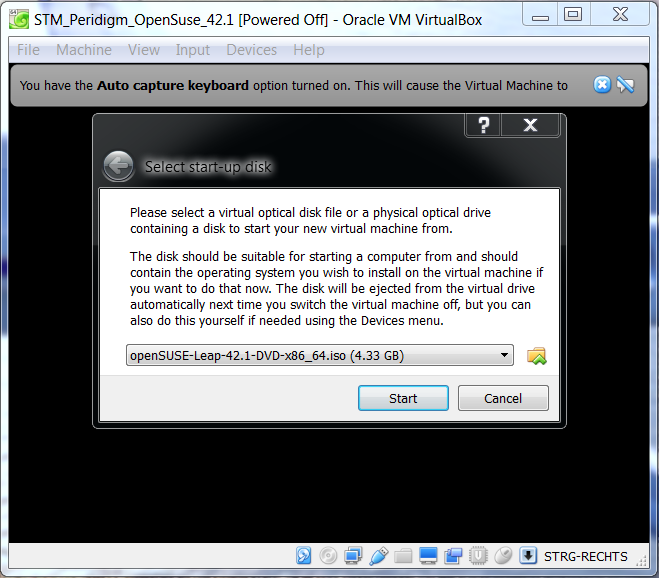
\includegraphics[scale=\screenshotscalefac]{Figures/VirtualBox_VirtualMachine_OperatingSystem_SelectDisk}
   \item Click \textit{Start}
 \end{itemize}
 \item Setup the installation
 \begin{itemize}
   \item In the \marktool{\opensusename} boot menu select \textit{Installation}\\
   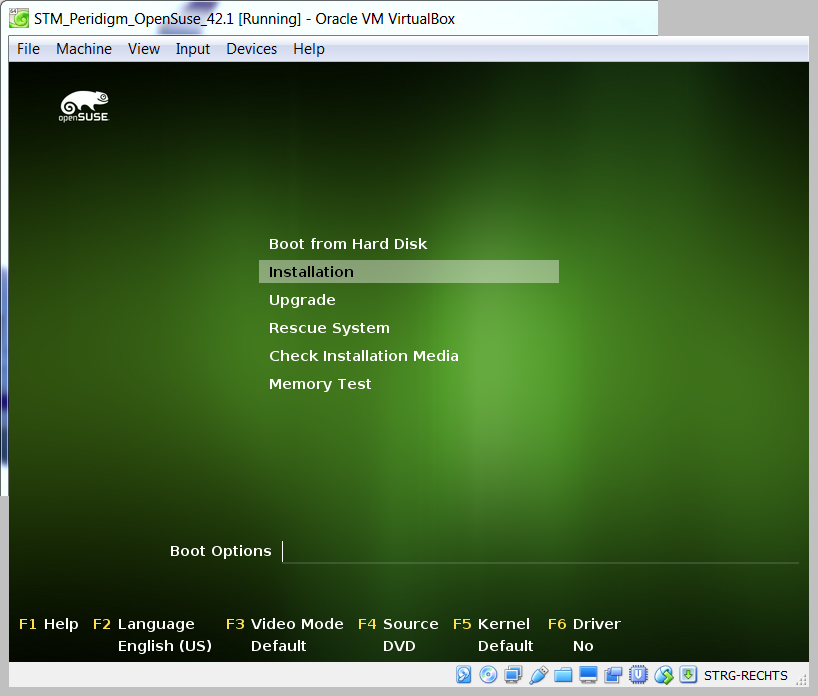
\includegraphics[scale=0.25]{Figures/VirtualBox_VirtualMachine_OperatingSystem_Boot_Installation}
   \item Set the Language and Keyboard layout to your preferred option\\
   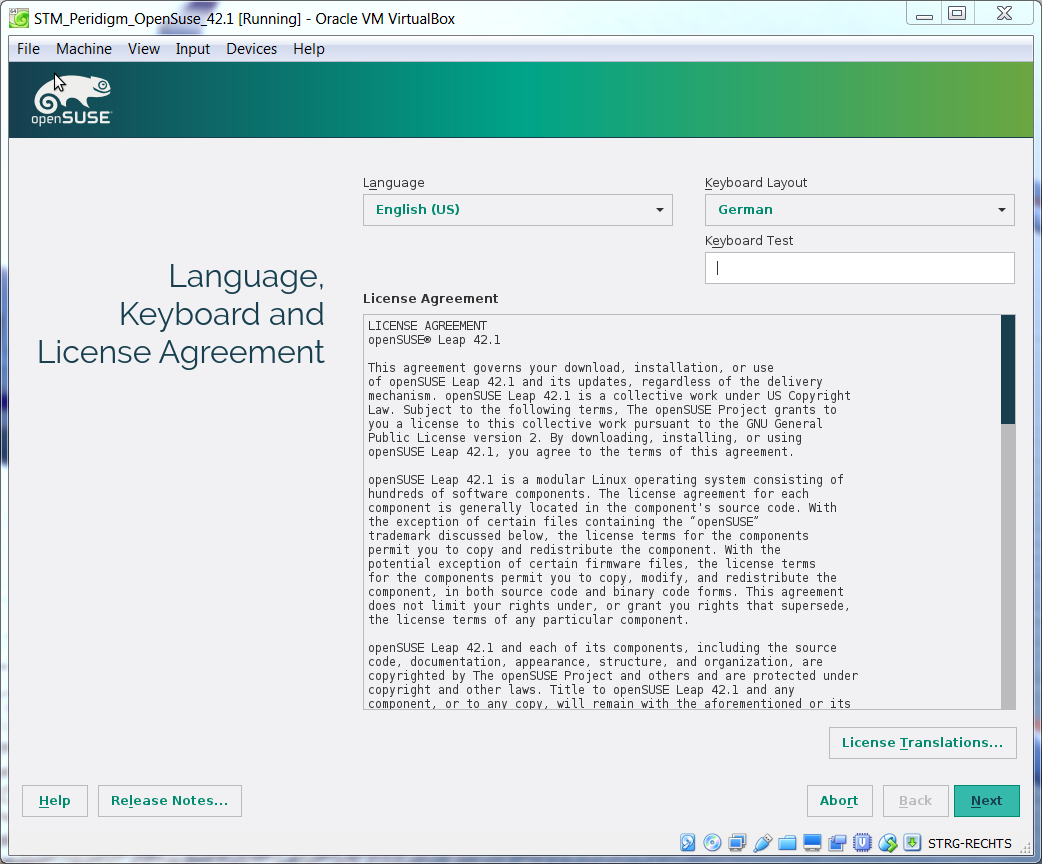
\includegraphics[scale=0.25]{Figures/VirtualBox_VirtualMachine_OperatingSystem_Language}
   \item Click \textit{Next}
   \item In the \textit{Installation Options} to not toggle on any of the options\\
   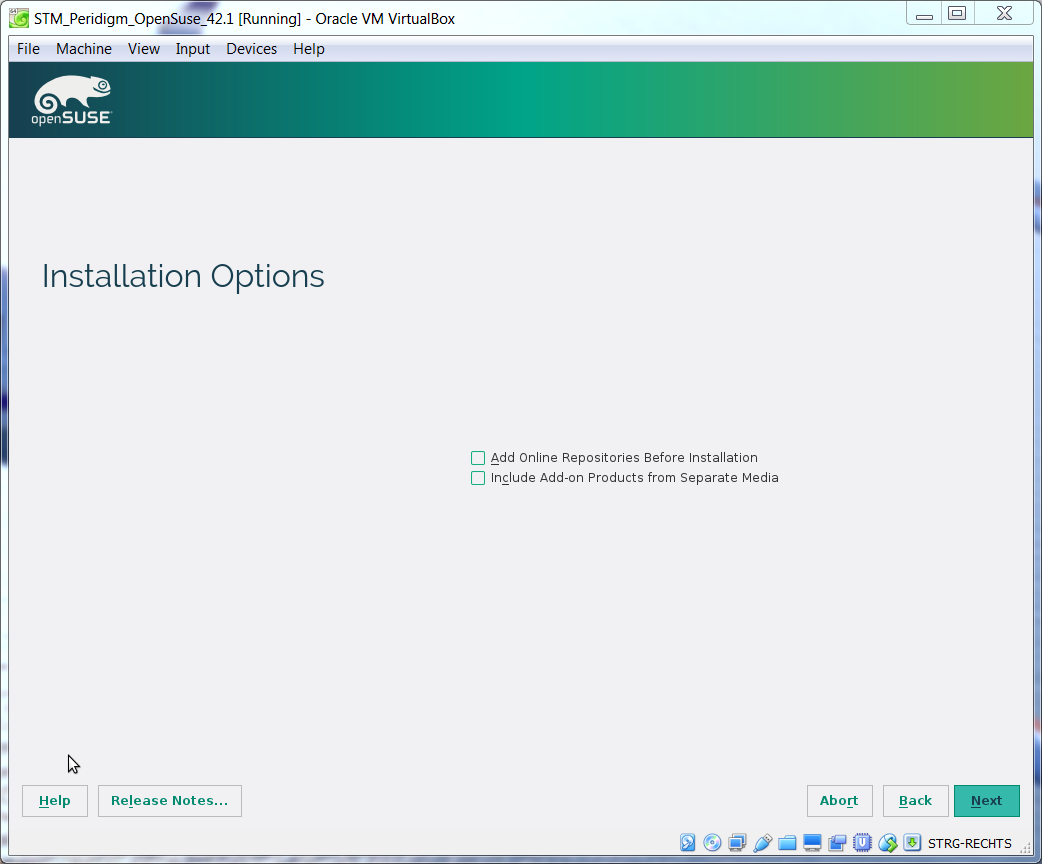
\includegraphics[scale=0.25]{Figures/VirtualBox_VirtualMachine_OperatingSystem_InstallationOptions}
   \item Click \textit{Next}
   \item Use the \textit{Suggested Partition} and click \textit{Next}
   \item Click on the Map to select your country to set \textit{Clock and Time Zone} and click \textit{Next}
   \item Use \textit{KDE Desktop} in \textit{Desktop Selection} and click \textit{Next}\\
   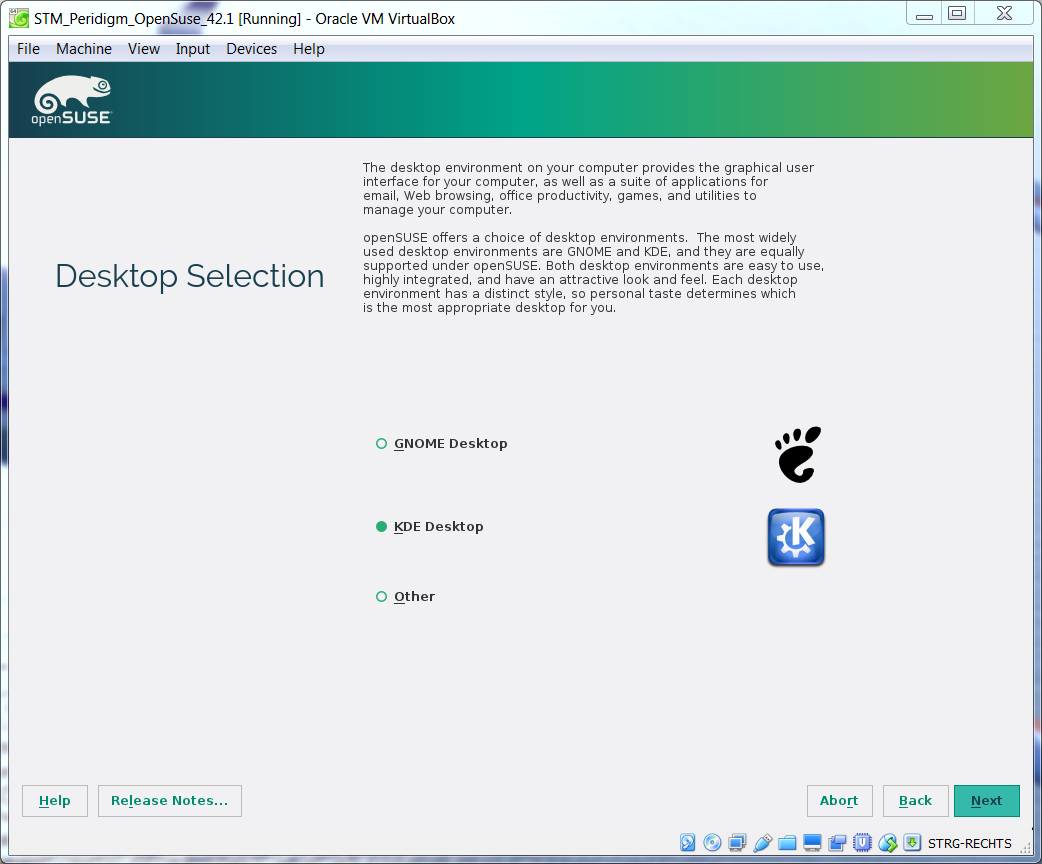
\includegraphics[scale=0.25]{Figures/VirtualBox_VirtualMachine_OperatingSystem_DesktopSelection}
   \item Setup the first user name \& password
   \begin{itemize}
    \item You can use the same user and root password if you are and will always be the only user of your virtual machine
    \item User: 
      \begin{tabular}[t]{ll}
      \textit{Username}	& stm	\\
      \textit{Password}	& 13112	\\
      \end{tabular}
    \item Admin:
      \begin{tabular}[t]{ll}
      \textit{Password}	& dlr-fa-13112-bs	\\
      \end{tabular}
    \item Click next
   \end{itemize}
   \item In the next windows click \textit{Install}
 \end{itemize}
 \item After installation
 \begin{itemize}
   \item After the installation is complete virtual system restarts. Now select \textit{Boot from Hard Disk}\\
   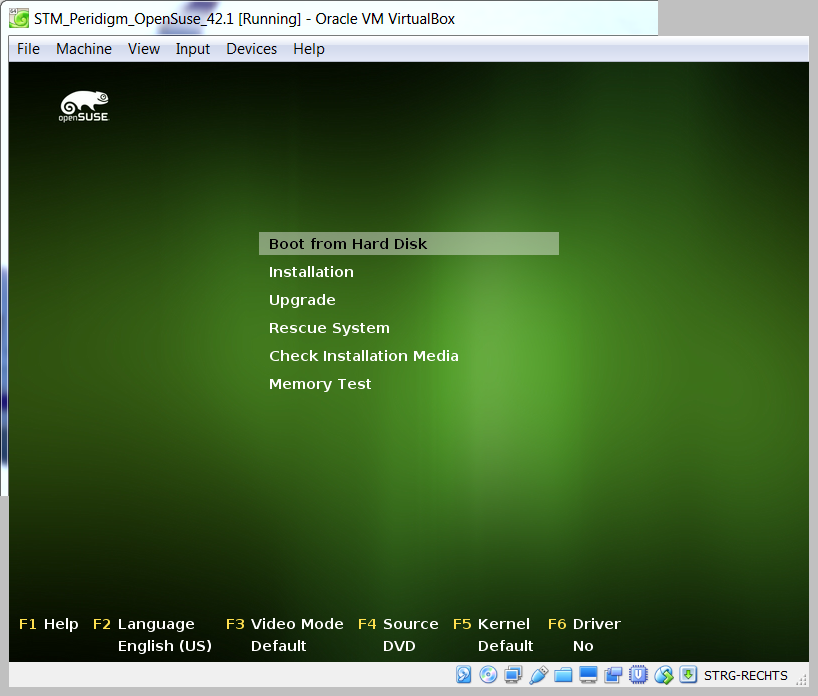
\includegraphics[scale=0.25]{Figures/VirtualBox_VirtualMachine_OperatingSystem_Boot_HardDisk}
   \item Select the normal version and press Enter\\
   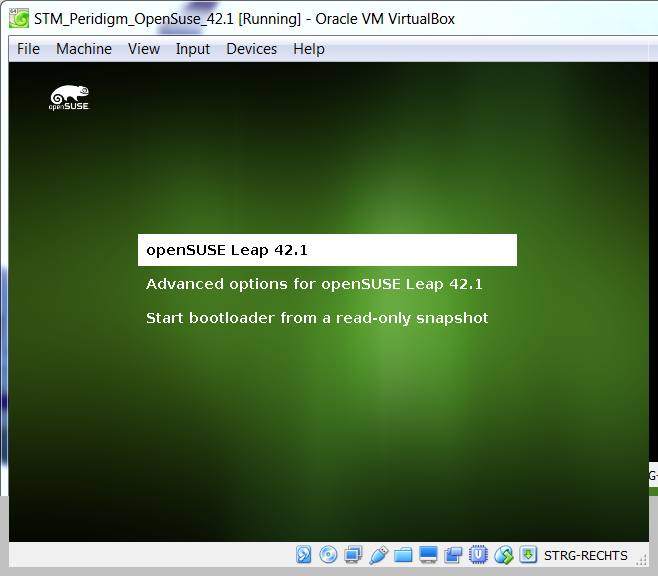
\includegraphics[scale=0.25]{Figures/VirtualBox_VirtualMachine_OperatingSystem_Boot_Version}
   \item Login with your password\\
   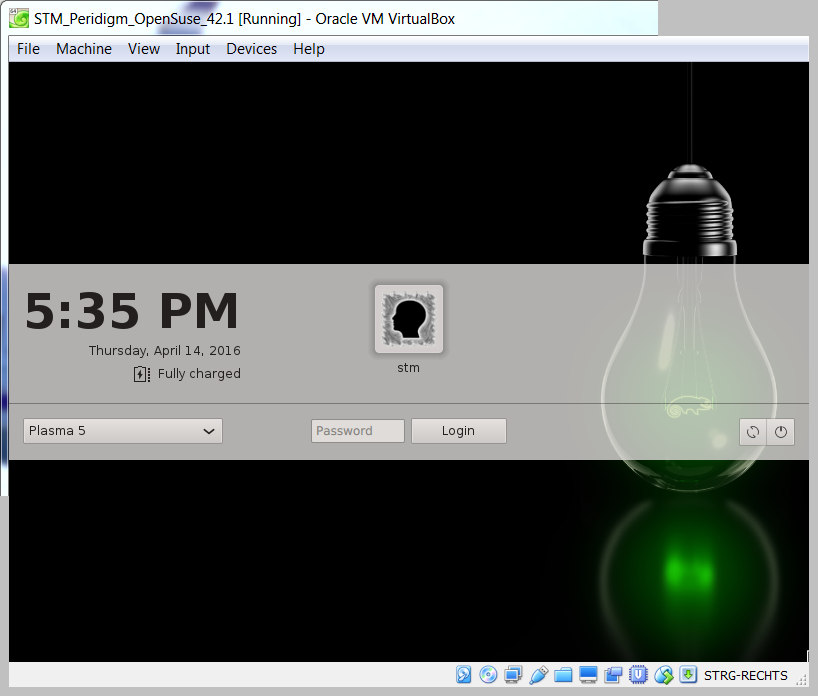
\includegraphics[scale=0.25]{Figures/VirtualBox_VirtualMachine_OperatingSystem_Login}
   \item Open a shell
   \item Login as root user, perform
\begin{code}
zypper refresh
zypper update
\end{code}
   And select yes to perform an operating system update
   \item Restart the virtual machine operating system
 \end{itemize}
\end{enumerate}

Ta-daa you have a linux installation inside of a virtual machine.

\levelstay{User modifications to use shared folders}

In order for the Linux users to use the virtual machine shared folders

\begin{enumerate}[noitemsep]
 \item Open \marktool{\yastname}
 \item In the \textit{Security and Users} tab open {User and Group Management}
 \item Select the user and click \textit{Edit}
 \item Go to \textit{Details} tab
 \item On the right select \textit{users} and \textit{vboxsf} as \textit{Additional Groups} and click \textit{OK}
 \item Restart your virtual system
\end{enumerate}

The shared folders are mounted under \verb+/media/+. In the current case the single shared folder is accessible under \verb+/media/sf_transfer/+ .

\levelstay{Save the virtual machine state}

After the operating system installation it is recommended to save a snapshot of the current virtual machine state. Thus, it is always possible to reset your virtual machine to this state in case anything goes wrong during the \marktool{\toolname} installation.

To create a snapshot:

\begin{enumerate}[noitemsep]
 \item Open the \marktool{\virtualboxname} Manager
 \item In the upper right corner select \textit{Snapshots}
 \item Click the little camera button to take a snapshot of the current virtual machine state\\
 \begin{tikzpicture}
   % External figure
   \node[anchor=south west,inner sep=0] (image) at (0,0){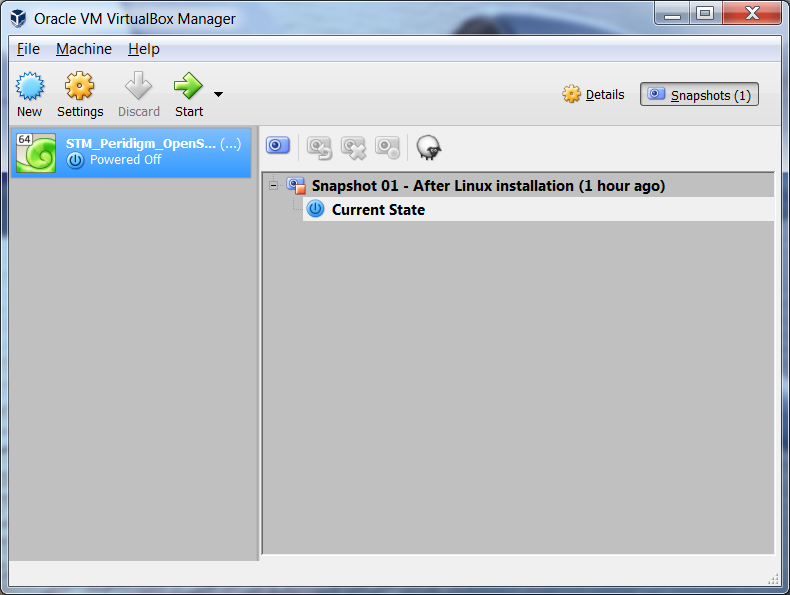
\includegraphics[scale=\screenshotscalefac]{Figures/VirtualBox_VirtualMachine_Snapshot}};
   % Figure scope
   \begin{scope}[
     x={(image.south east)},
     y={(image.north west)},
   ]
     % Red rectangle
     \draw[red,ultra thick,rounded corners] (0.325,0.73) rectangle (0.3775,0.786);
     % Help grid and labels
%      \pic{myimagegrid};
   \end{scope}
 \end{tikzpicture}
 
\end{enumerate}
